\documentclass[compress]{beamer}
\usepackage{ifthen,verbatim,ulem}

\title{Optimizing the corrected alignment procedure}
\author{Jim Pivarski}
\institute{Texas A\&M University}
\date{20 November, 2007}

\newcommand{\isnote}{}
\xdefinecolor{lightyellow}{rgb}{1.,1.,0.25}
\xdefinecolor{darkblue}{rgb}{0.1,0.1,0.7}

%% Uncomment this to get annotations
%% \def\notes{\addtocounter{page}{-1}
%%            \renewcommand{\isnote}{*}
%% 	   \beamertemplateshadingbackground{lightyellow}{white}
%%            \begin{frame}
%%            \frametitle{Notes for the previous page (page \insertpagenumber)}
%%            \itemize}
%% \def\endnotes{\enditemize
%% 	      \end{frame}
%%               \beamertemplateshadingbackground{white}{white}
%%               \renewcommand{\isnote}{}}

%% Uncomment this to not get annotations
\def\notes{\comment}
\def\endnotes{\endcomment}

\setbeamertemplate{navigation symbols}{}
\setbeamertemplate{headline}{\includegraphics[height=1 cm]{../cmslogo} \hspace{0.1 cm} \includegraphics[height=1 cm]{../tamulogo} \hfill
\begin{minipage}{5.5 cm}
\vspace{-0.75 cm} \small
\begin{center}
\ifthenelse{\equal{\insertpagenumber}{1}}{}{\textcolor{blue}{\insertsection}}
\end{center}
\end{minipage} \hfill
\begin{minipage}{4.5 cm}
\vspace{-0.75 cm} \small
\begin{flushright}
\ifthenelse{\equal{\insertpagenumber}{1}}{}{Jim Pivarski \hspace{0.5 cm} \insertpagenumber\isnote/\pageref{numpages}}
\end{flushright}
\end{minipage}\mbox{\hspace{0.2 cm}}}

\begin{document}
\frame{\titlepage}

%% \begin{notes}
%% \item This is the annotated version of my talk.
%% \item If you want the version that I am presenting, download the one
%% labeled ``slides'' on Indico (or just ignore these yellow pages).
%% \item The annotated version is provided for extra detail and a written
%% record of comments that I intend to make orally.
%% \item Yellow notes refer to the content on the {\it previous} page.
%% \item All other slides are identical for the two versions.
%% \end{notes}

\begin{frame}
\frametitle{In this talk}
\begin{enumerate}\setlength{\itemsep}{0.75 cm}
\item New three-pass procedure
\item Optimizing Alignment Parameter Errors (APEs) in a 1-dimensional setting
\item Optimizing degrees of freedom in a 6-dof setting, with application to TeV muons
\end{enumerate}

\vfill
This is a work-in-progress talk: how things are going, rather than final results
\end{frame}

\section*{New three-pass procedure}

\begin{frame}
\frametitle{Why not align everything at once?}

\textcolor{darkblue}{Problem:} tracks emerge from calorimeter/solenoid with more uncertainty
than they do when passing through the iron between stations, so
we get a poor alignment if we let everything float at once

\vspace{-0.35 cm}
\begin{center}
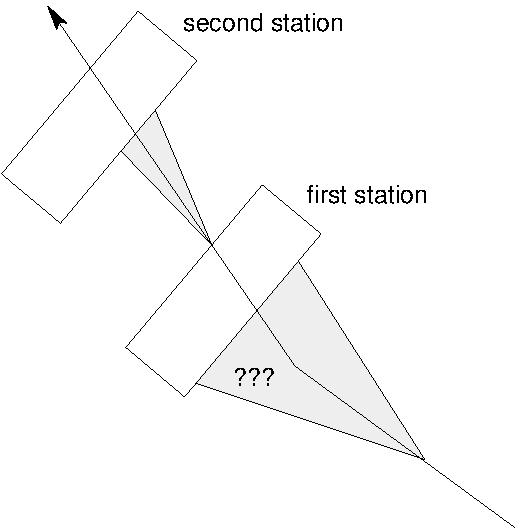
\includegraphics[width=0.35\linewidth]{problemsolution.pdf}
\end{center}

\vspace{-0.35 cm}
\textcolor{darkblue}{Solution:} align the outer stations only after
the inner stations are well-placed: at least two passes
\end{frame}

\begin{frame}
\frametitle{The current procedure}

\begin{enumerate}\setlength{\itemsep}{0.25 cm}
\item Align muon barrel station 1 (MB1) and endcap stations ME1/1 and
ME1/2 with 2~cm APEs (loose), all other muon stations have 5~cm (very
loose).

\vspace{0.25 cm}
{\it At this point, the inner stations are aligned to 400--500~$\mu$m.)

\item Align all other stations (MB1, ME1/1, and ME1/2 are now {\it
fixed}) with 5~mm APEs.}

\vspace{0.25 cm} {\it At this point, the outer stations are aligned to
400--800~$\mu$m, with MB4 and ME4/1 having the worst resolution:
1.5~cm.  Chambers probably have better relative alignments
than global alignments.}

\item Try to align groups of internally-aligned chambers to the
tracker by re-aligning everything with 500~$\mu$m APEs.

\end{enumerate}
\end{frame}

\begin{frame}
\frametitle{How APEs were optimized}

Start with artificial misalignments: all chambers in a station (MB1
here) are moved 1~cm, chambers in other stations are
Gaussian-distributed.

\vspace{0.1 cm}
Each chamber is realigned independently: plot mean and stdev

\begin{center}
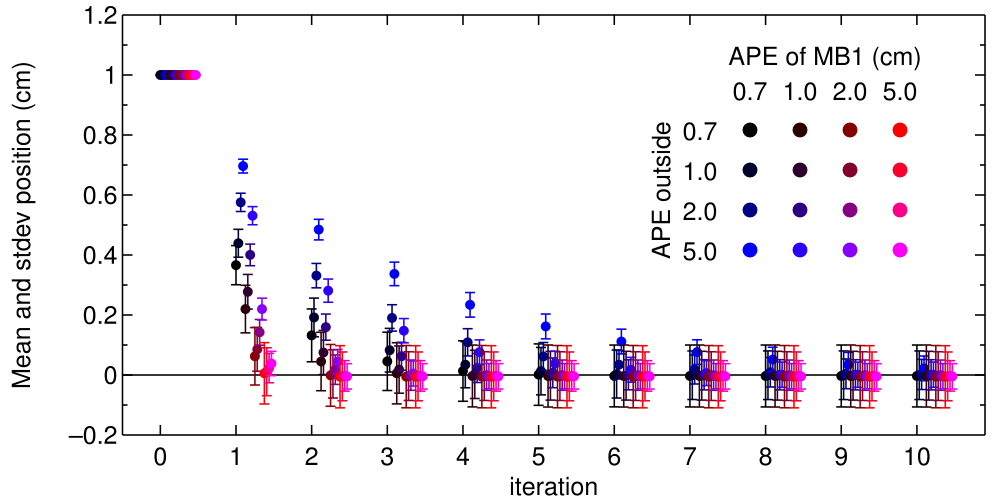
\includegraphics[width=0.8\linewidth]{mb1_meanstdev.png}
\end{center}
\end{frame}

\section*{Alignment results}

\begin{frame}
\frametitle{Alignment results: general 1-dimensional}

Now we do more a realistic alignment with all chambers randomly
distributed $\pm$5~mm, but still 1-dimensional (local $x$).

\vspace{0.25 cm}
Alignment resolution of $x$ in microns (stages 1\&2 only):

\begin{tabular}{r l r l r l r l}
MB1 & 430 & MB2 & 400 & MB3 & 700 & MB4 & 1174 \\
ME1/2 & 380 & ME1/3 & 340 & ME2/2 & 510 & ME3/2 & \textcolor{white}{0}730 \\
ME1/1 & 520 & ME2/1 & 620 & ME3/1 & 850 & ME4/1 & 1030 \\
\end{tabular}

\vspace{0.5 cm}
Alignment resolution {\it if inner chambers were perfectly aligned}

\begin{tabular}{r l r l r l r l}
MB1 & 430 & MB2 & 70 & MB3 & 120 & MB4 & 160 \\
ME1/2 & 380 & ME1/3 & 190 & ME2/2 & 200 & ME3/2 & 230 \\
ME1/1 & 520 & ME2/1 & 270 & ME3/1 & 120 & ME4/1 & 130 \\
\end{tabular}

\vspace{0.25 cm} (There's still a significant problem with propagating
errors through the system, mostly at the third step: maybe I should
revisit the idea of one pass for each station\ldots)
\end{frame}

\section*{Degree of freedom optimization}

\begin{frame}
\frametitle{More general misalignments:}
\begin{itemize}\setlength{\itemsep}{0.25 cm}
\item Misalign chambers uniformly $\pm$5~mm, $\pm$5~mrad in all directions (very messy starting point!)
\item No wheel/disk misalignments yet (I expect that to be easy)
\item Assume that the optimal 1-dof APEs optimize the 6-dof problem
\item Allow various parameters to float
\begin{itemize}
\item MB1--3 (good $y$ measurement): drop all combinations of $z$ and $\phi_x$
\item MB4 (no $y$ measurement): certainly drop $y$ and $\phi_x$, maybe drop $z$
\item ME (poor $y$ measurement): probably drop $z$, $\phi_x$, and maybe even $\phi_y$
\end{itemize}
\item Determine alignment quality from TeV $p_T$ resolution
\end{itemize}

\end{frame}

\begin{frame}
What was allowed to float \hfill 2~TeV track resolutions \\
\hfill through $\eta$ ranges (in \% of $p_T$)

\vspace{0.2 cm}
\begin{minipage}{1.1\linewidth}
\small
\begin{tabular}{c c c | c c c c}
MB1--3 & MB4 & ME & barrel & ME1/3 & ME1/2 & ME1/1 \\\hline

ideal & ideal & ideal & 5.3  &  4.9  &  5.0  &  5.9  \\\hline

$xy..\phi_y\phi_z$ & $x...\phi_y\phi_z$ & $xyz\phi_x\phi_y\phi_z$ &  6.4  &  6.1  &  6.1  &  6.7  \\
$xy..\phi_y\phi_z$ & $x.z.\phi_y\phi_z$ & $xyz\phi_x\phi_y\phi_z$ &  6.4  &  6.1  &  6.1  &  6.6  \\
$xy.\phi_x\phi_y\phi_z$ & $x...\phi_y\phi_z$ & $xyz\phi_x\phi_y\phi_z$ &  6.3  &  6.2  &  6.0  &  6.5  \\
$xyz.\phi_y\phi_z$ & $x...\phi_y\phi_z$ & $xyz\phi_x\phi_y\phi_z$ &  6.2  &  5.8  &  6.2  &  6.4  \\
$xyz.\phi_y\phi_z$ & $x.z.\phi_y\phi_z$ & $xyz\phi_x\phi_y\phi_z$ &  6.2  &  5.8  &  6.2  &  6.2  \\
$xyz\phi_x\phi_y\phi_z$ & $x...\phi_y\phi_z$ & $xyz\phi_x\phi_y\phi_z$ &  6.2  &  5.8  &  6.0  &  6.2  \\
$xyz\phi_x\phi_y\phi_z$ & $x.z.\phi_y\phi_z$ & $xyz\phi_x\phi_y\phi_z$ &  6.1  &  5.8  &  6.0  &  6.2  \\\hline

$xyz\phi_x\phi_y\phi_z$ & $x.z.\phi_y\phi_z$ & $xyz\phi_x\phi_y\phi_z$ &  6.1  &  5.8  &  6.0  &  6.2  \\
$xyz\phi_x\phi_y\phi_z$ & $x.z.\phi_y\phi_z$ & $xy...\phi_z$ &  6.1  &  5.7  &  6.0  &  6.6  \\
$xyz\phi_x\phi_y\phi_z$ & $x.z.\phi_y\phi_z$ & $xy..\phi_y\phi_z$ &  6.1  &  5.7  &  5.9  &  6.5  \\
$xyz\phi_x\phi_y\phi_z$ & $x.z.\phi_y\phi_z$ & $xy.\phi_x\phi_y\phi_z$ &  6.1  &  5.8  &  5.9  &  6.6  \\
\end{tabular}
\end{minipage}

\vspace{0.2 cm} Conclusion: it doesn't make much difference, but allowing more to float is slightly better.
\end{frame}

\begin{frame}
\frametitle{Results for best scenario}

\vspace{-0.8 cm} \hfill {\scriptsize (MB1-3 $xyz\phi_x\phi_y\phi_z$ MB4 $x.z.\phi_y\phi_z$ ME $xyz\phi_x\phi_y\phi_z$) \mbox{\hspace{-0.25 cm}}}

\vspace{0.4 cm}
\hspace{-0.83 cm} \textcolor{darkblue}{Stages 1\&2 only (mm and mrad):}

\begin{tabular}{c c c c c c c}
\mbox{ } & $x$ & $y$ & $z$ & $\phi_x$ & $\phi_y$ & $\phi_z$ \\
barrel & 0.94 & 2.1 & 2.6 & 2.0 & 0.87 & 0.78 \\
endcap & 0.91 & 3.5 & 4.0 & flat 5~mm & 1.5 & 1.2
\end{tabular}

\vspace{0.5 cm}

\hspace{-0.83 cm} \textcolor{darkblue}{Stage 3 (small APE align everything):}

\begin{tabular}{c c c c c c c}
\mbox{ } & $x$ & $y$ & $z$ & $\phi_x$ & $\phi_y$ & $\phi_z$ \\
barrel & 0.81 & 2.0 & 2.4 & 2.0 & 0.70 & 0.63 \\
endcap & 0.85 & 3.5 & 4.0 & flat 5~mm & 1.1 & 1.1
\end{tabular}

\vspace{0.2 cm}
\begin{itemize}
\item Stage 3 does help in $x$ and $\phi_z$ (the most important parameters)
\item Let's not align endcap $z$ or $\phi_x$; they're not really converging in 10~pb$^{-1}$
\end{itemize}
\end{frame}

\section*{Conclusions}

\begin{frame}
\frametitle{The Bottom Line!}
Reconstructed 2~TeV $Z'$ from scratch using the new alignments: this is our latest 10~pb$^{-1}$ scenario
\begin{center}
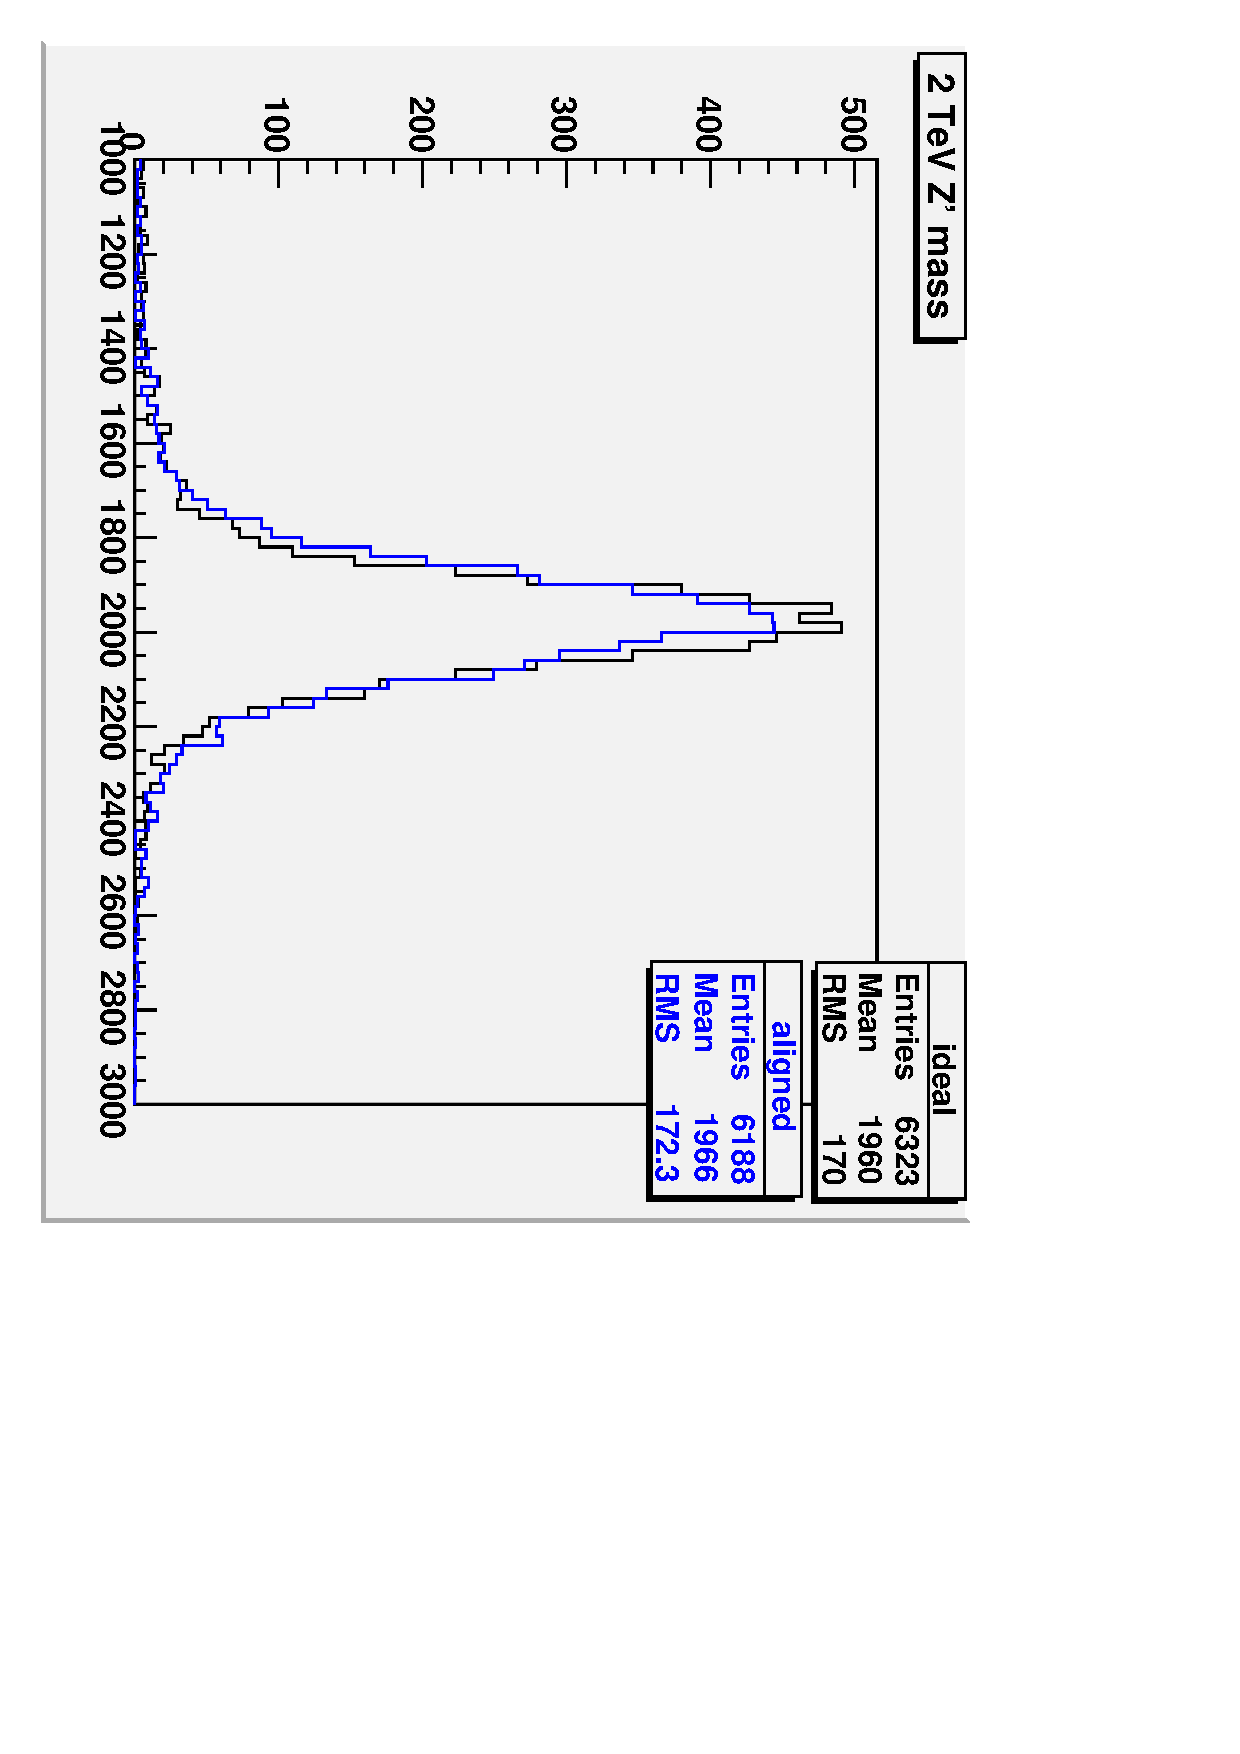
\includegraphics[height=0.75\linewidth, angle=90]{zprime_peak.pdf}
\end{center}
\end{frame}

\begin{frame}
\frametitle{Comments on the bottom line}
\begin{center}
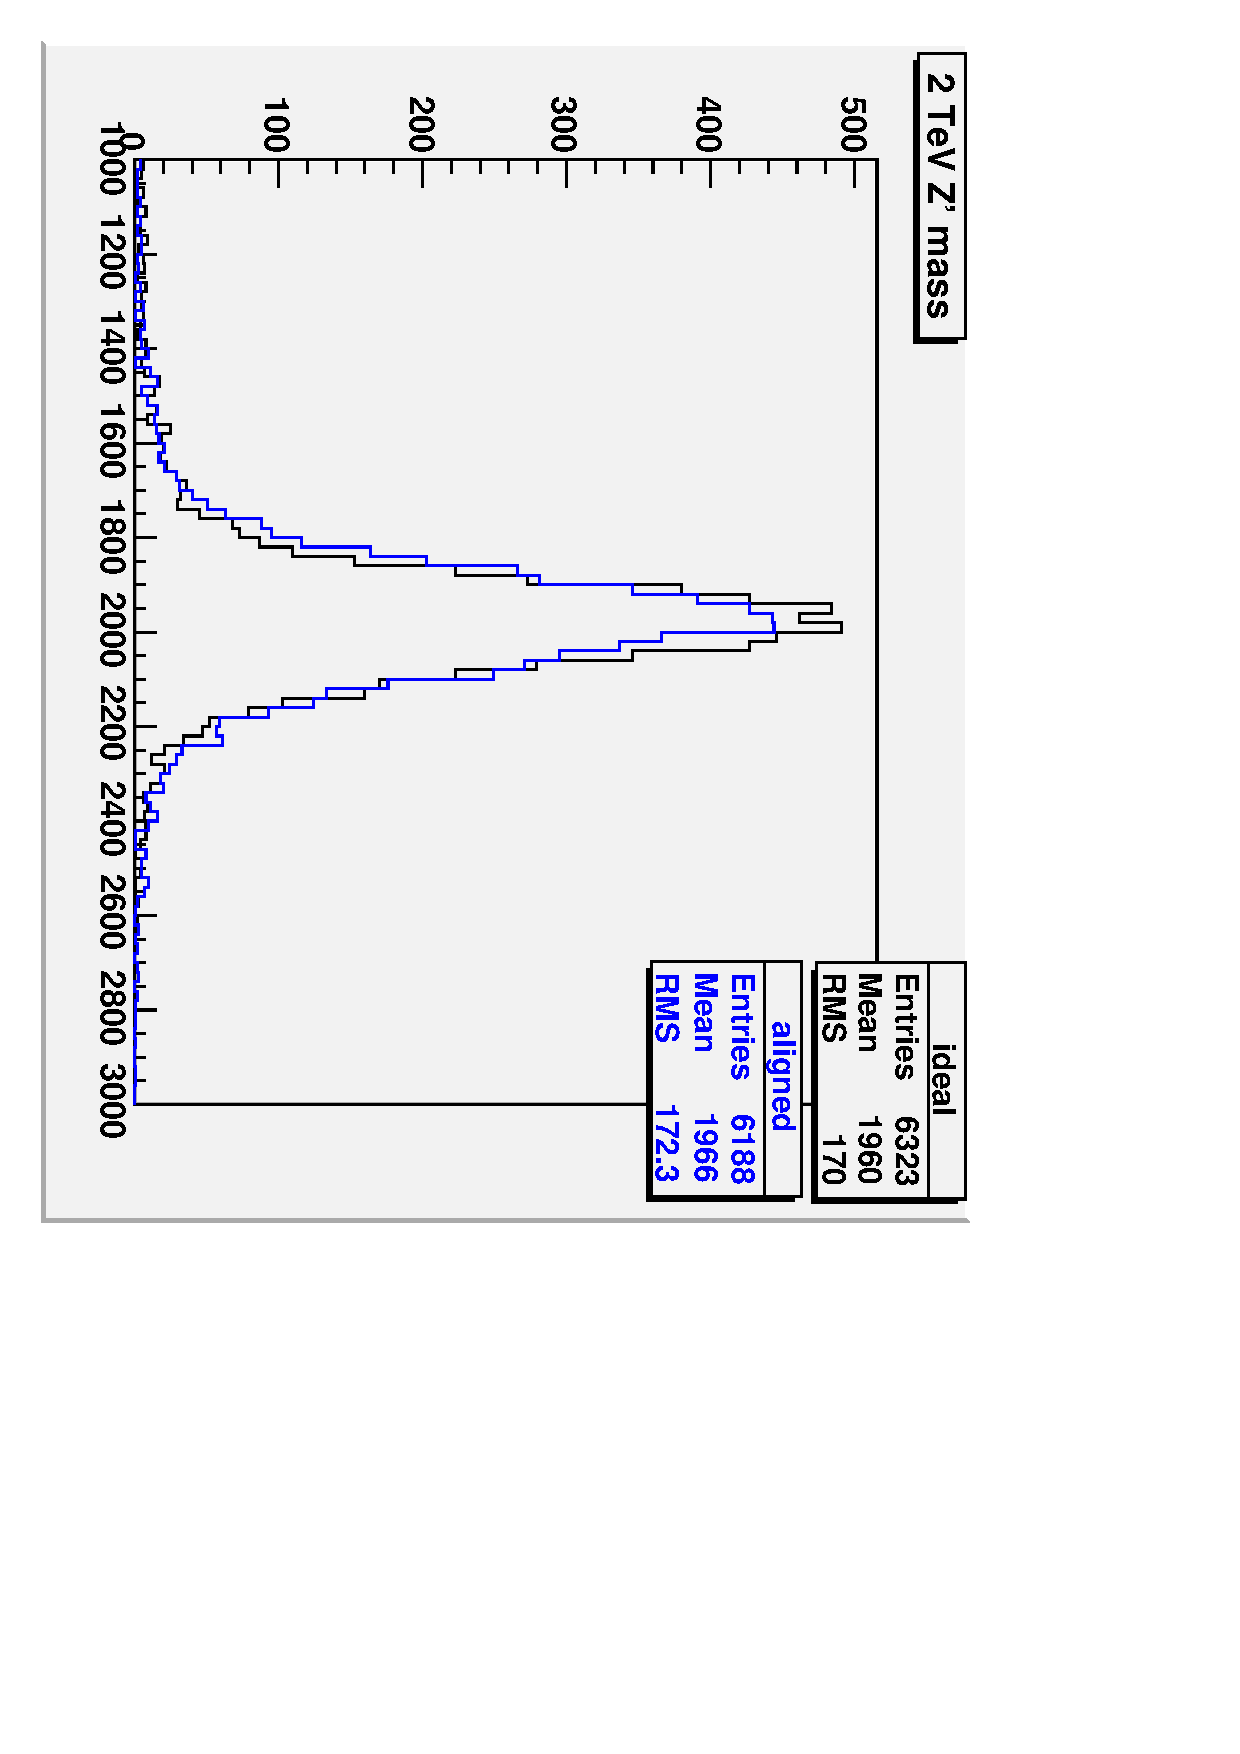
\includegraphics[height=0.25\linewidth, angle=90]{zprime_peak.pdf}
\end{center}
\begin{itemize}
\item Still much better than standard muon alignment scenario (which
has about $\frac{1}{2}$ the resolution of ideal)
\item Standard scenario has 500~$\mu$m chamber errors and
2--5~mm wheel/disk errors; our simulation had no wheel/disk misalignments
\item Time to try wheel/disk alignments in the new procedure!
\item The track-finding efficiency is 2\% lower with misalignment
\item Baseline track-finding efficiency is 94\% (Dubna group)
\end{itemize}
\label{numpages}
\end{frame}

\end{document}
